\documentclass[11pt, a4paper]{article}

\usepackage{amsmath}
\usepackage{amsfonts} %Matheschriften
\usepackage{amssymb} %Mathesymbole
%\usepackage{mathptmx} % Einstellung für Schriften und Sonderzeichen in mathematischen Umgebungen
                        % ändert SChriftfont
\usepackage{wasysym} % Stellt diverse Sonderzeichen bereit
\usepackage{siunitx}
\usepackage{float}
\usepackage{microtype}
\usepackage{graphicx}
\usepackage{hyperref}
\usepackage{xcolor}
\usepackage[section]{placeins}
% allows for temporary adjustment of side margins
\usepackage{changepage}
\usepackage{rotating}


\usepackage[ngerman]{babel}
\addto\captionsngerman{%
 \renewcommand{\abstractname}{Einleitung}}

\title{Versuch 4: Transistor}
\author{Team 2-13: Jascha Fricker, Benedict Brouwer}

\begin{document}
    \maketitle

    \tableofcontents

    \newpage
\section{Introduction}
In this experiment we examined the properties of a bipolar transistor in combination with an emitter circuit. Therby we measured the characteristic curve 
of the transistor and tested different konfigurations of the emittercircuit.
\section{Theorie}

\subsection{small signal model}
For small deviations around the workingpoint one can use the small signal modell leading to the following equation.
\begin{align}
\left(\begin{array}{l}
    d I_{\mathrm{B}} \\
    d I_{\mathrm{C}}
    \end{array}\right)=\left(\begin{array}{cc}
    \frac{1}{r_{\mathrm{BE}}} & S_{\mathrm{r}} \\
    S & \frac{1}{r_{\mathrm{CE}}}
    \end{array}\right)\left(\begin{array}{l}
    d U_{\mathrm{BE}} \\
    d U_{\mathrm{CE}}
    \end{array}\right)
\end{align}

whereby $r_{\text{BE}}$, $r_{\text{CE}}$ and the steepness $S$ can be calculated with
\begin{align}
    \frac{1}{r_{\text{BE}}} = \frac{\partial I_{\text{B}}}{\partial U_{\text{BE}}} |_{U_{\text{CE}}} \label{eq:rbe} \\ \\
    \frac{1}{r_{\text{CE}}} = \frac{\partial I_{\text{C}}}{\partial U_{\text{CE}}} |_{U_{\text{BE}}} \label{eq:rce} \\ \\
    S=\left .\frac{\partial I_{\mathrm{C}}}{\partial U_{\mathrm{BE}}}\right |_{U_{\mathrm{CE}}}=\frac{q I_{\mathrm{C}}}{k_{\mathrm{B}} T} \label{eq:steep}
\end{align}

In addition to that $I_{\mathrm{B}}$ can be calculated the following proportionality 
\begin{align}
    I_{\mathrm{B}} \propto \exp \left(\frac{q U_{\mathrm{BE}}}{k_{\mathrm{B}} T}\right)
    \label{eq:Ib_T}
    
\end{align}





\section{execution}
\begin{figure}[h]
    \centering
    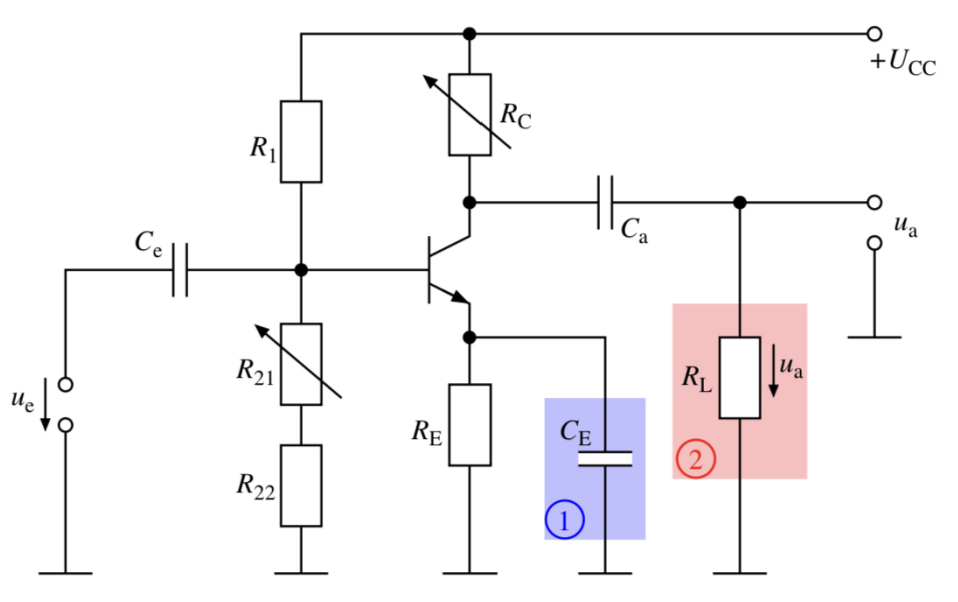
\includegraphics[width=0.8\textwidth]{bilder/Emitter circuit.png}
    \caption{emittercircuit:\\
    $R_1$ = 47 \si{\kilo\ohm}, $R_{22}$ = 100 \si{\ohm},$R_E$ = 10 \si{\kilo\ohm}, $C_e$ = 47 \si{\micro\farad},$C_a$ = 470 \si{\micro\farad}, $U_{CC}$ = 9 \si{\volt} 
    $R_{12}$: potentiometer for the workingpoint, $R_C$: potentiometer 0 - 10 \si{\kilo\ohm}, $u_e$: inputvoltage, $u_a$: outputvoltage
    
    }
    \label{im:Emcir}
\end{figure}

\subsection{workingpoint}
A bipolar transistor has a specific basevoltage range (the so called workingpoint) in wich it behaves approxmately linear. This workingpoint
is tuned by setting the resistance at the potentiometer $R_{12}$ \ref{im:Emcir}[see circuit diagram] to a point whereby the outputamplitude $u_a$ is maximal and the signal is not distorted.
To tune the workingpoint, the loadresistor $R_L$ was removed and a sinusoidal frequency of 5.5 \si{\kilp\hertz} was applied. 
$U_{\text{BE}}$, $U_{\text{CE}}$, $I_{\text{C}}$ where measured with varying $R_{\text{C}}$ for further evaluation.
\subsection{Amplification of the emittercircuit}
To further examine the emittercircuit \ref{im:Emcir}[see circuit diagram] the amplidude quotionet $u_a / u_e$ was measured for varying $R_{\text{C}}$ in different circuit configurations:\\
1. with capacitor $C{\text{E}}$ but without resistor $R_{\text{L}}$
2. without capacitor $C{\text{E}}$ and without resistor $R_{\text{L}}$
3. with capacitor $C{\text{E}}$ and resistor $R_{\text{L}}$
\subsection{Frequency response}
In this experiment the input frequency was varied from 6 \si{\hertz} - 250 \si{\kilo\hertz} to measure the phaseshift and the amplidude quotionet $u_a / u_e$. 
Therby circuit \ref{im:Emcir} with an collectorresistor of $R_{\text{C}}$ was used. In addition to that the oszilloscope was changed to x-y mode to observe lissajous curves.
\subsection{characteristic curve}
\begin{figure}[h]
    \centering
    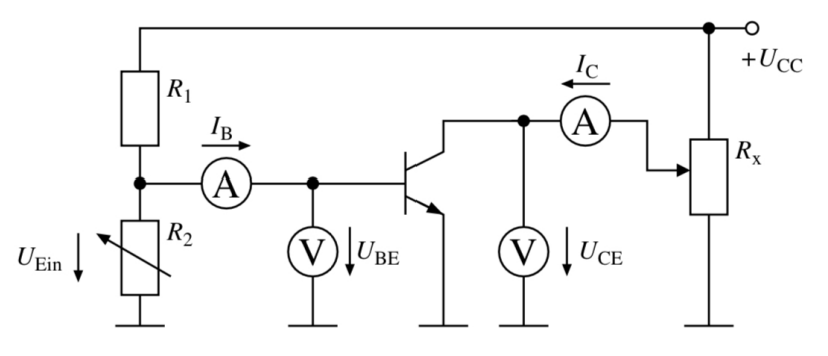
\includegraphics[width=0.8\textwidth]{bilder/characteristicCurve.png}
    \caption{characteristic curve \\
    $R_1$ = 1 \si{\kilo\ohm}, $R_2$ = 220 \si{\ohm}}
    \label{im:Charcurcir}
\end{figure}

To measure the characteristic curve of the transistor the circuit was change as shown in the circuit diagram \ref{im:Charcurcir}. 
First the entry curve $I_{\text{B}}=f(U_{\text{BE}})|_{U_{\text{CE}}}$ was taken by changing $U_{\text{BE}}$ from 0 to 670 \si{\milli\volt} and measuring $I_{\text{B}}$,
$U_{\text{BE}}$ and $U_{\text{CE}}$ with multimeters according to the scematic \ref{im:Charcurcir}. Therby $U_{\text{CE}}$ was dialed in to match the results from experiment 1 \ref{tab:workingpoint_measurement} with $R_{\text{C}}$ = 5 \si{\kilo\ohm}.
Afterwards the output characteristic curve $I_{\text{C}} = f(U_{\text{CE}})|_{U_{\text{BE}}}$ was recorded with a varying $U_{\text{CE}}$ from 1 - 10 \si{\volt} by measuring $I_{\text{C}}$, $U_{\text{BE}}$ and $U_{\text{CE}}$. This curve was measured in both directions to observe the effect of heat on the transistor.

\section{Evaluation and results}
\subsection{preliminary considerations}
\subsection{characteristic curve (Assignment 7)}
As shown in table \ref{tab:workingpoint_measurement} some basevalues where recorded wich were needed in following experiments. They seem to be in a reasonable range.

\begin{table}[H]
    \centering
    \begin{tabular}{C|C|C|C}
    
        $R_{\text{C}}$ in \si{\kilo\ohm}  & $U_{\text{BE}}$ in \si{\volt} & $U_{\text{CE}}$ in \si{\volt} & $I_{\text{C}}$ in \si{\milli\ampere} & $S$ in \si{1\per\ohm} \\ \hline
        1 & 0,57 & 7,86 & 0,58 & 0.025\\ 
        5 & 0,57 & 5,53 & 0,58 & 0.025\\ 
        10 & 0,57 & 3,22 & 0,58 & 0.025\\ 
    \end{tabular}
    \label{tab:workingpoint_measurement}
    \caption{Basevalues}
\end{table}

The characteristic input curve is plottet in figure \ref{fig:Eincur}. With the slope from the tangent one can calculate the Baseresistance $r_{\text{BE}}$ = 3.92 \si{\kilo\ohm} with equation \ref{eq:rbe}
and the operating temperature $T$ = 272,2 \si{\kelvin} can obtained by using the fitparameters from the exponetial fit and equation \ref{eq:Ib_T}. Althoug the operating temperature has the correct magnitude it schould be at least 30 \si{\kelvin} higher.
With this operating temperature and equation \ref{eq:steep} the steepness $S$ can be calculated as shown in figure \ref{tab:workingpoint_measurement}.

\begin{figure}[h]
    \centering
    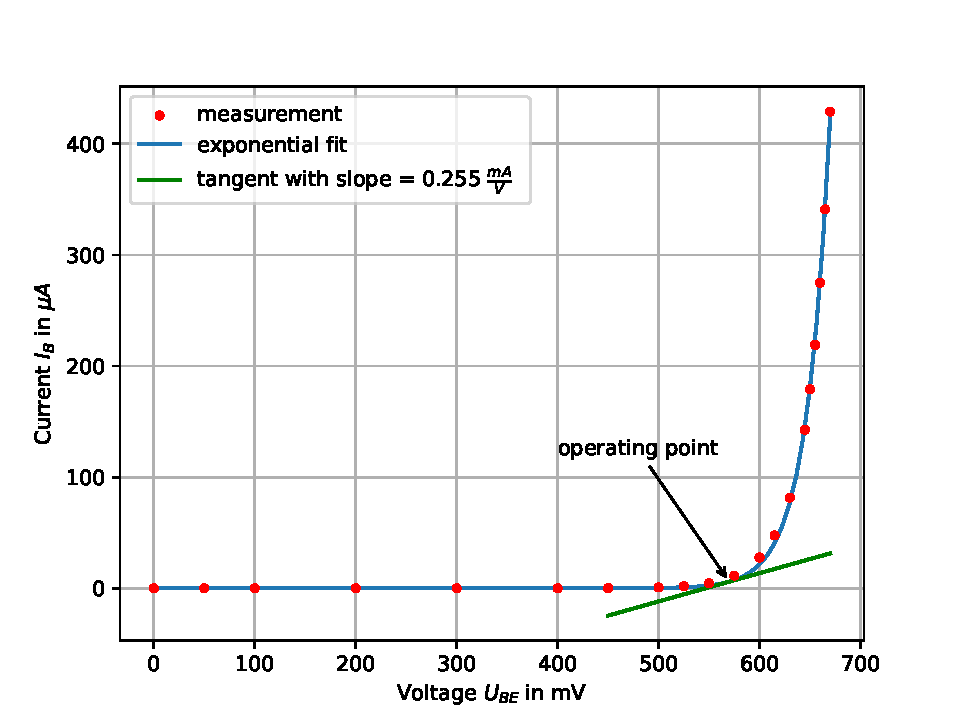
\includegraphics[width=0.8\textwidth]{plots/Eingangskennlinie.pdf}
    \caption{Characteristic curve from the input}
    \label{fig:Eincur}
\end{figure}

\begin{figure}[h]
    \centering
    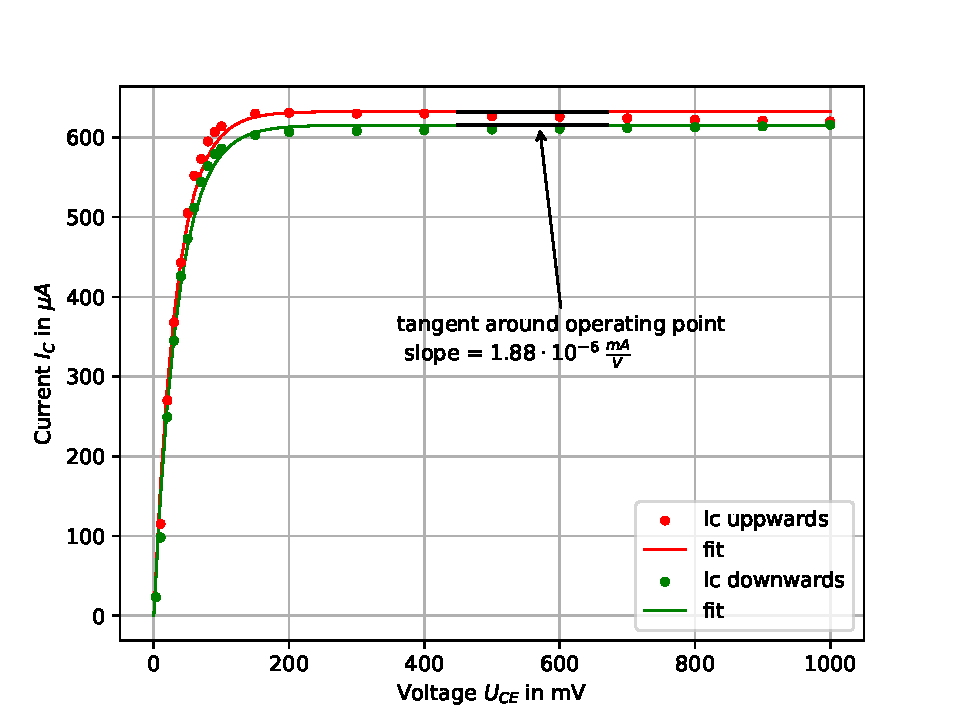
\includegraphics[width=0.8\textwidth]{plots/Ausgangskennlinie.pdf}
    \caption{Characteristic curve from the output}
    \label{fig:Outcur}
\end{figure}





\bibliographystyle{plain}
\bibliography{literature}

\end{document}

